% Online Resource 1 (electronic supplementary material) for the Journal of Intelligent Information Systems manuscript.
% Build: tectonic supplementary.tex   (or python JIIS/make_submission.py, which builds all upload files)
% Springer publishes supplementary files as received, so this is a plain A4 PDF; Springer asks that it name the article, journal, authors and corresponding author.
% Anonymized for double-blind review: restore the author block and the repository link in sections/appendix.tex at acceptance.
% Tables are numbered S1-S13 and the figure S1; the main text refers to them by these numbers, and this file refers to the main tables by number.
\documentclass[10pt,a4paper]{article}

\usepackage[margin=2cm]{geometry}
\usepackage[T1]{fontenc}
\usepackage{amsmath,amssymb}
\usepackage{booktabs}
\usepackage{multirow}
\usepackage{graphicx}
\usepackage[figuresright]{rotating}
\usepackage{url}
\usepackage[numbers,sort&compress]{natbib}
\usepackage[colorlinks,citecolor=blue,urlcolor=blue,linkcolor=blue]{hyperref}

\renewcommand{\thetable}{S\arabic{table}}
\renewcommand{\thefigure}{S\arabic{figure}}
% defined by sn-jnl, which the main article uses with sn-basic.bst
\providecommand{\bibcommenthead}{}

\begin{document}

\begin{center}
{\Large\bfseries Online Resource 1\par}
\vspace{0.5em}
{\large Typed Decision Models as Passage Rerankers: Effectiveness, Calibration, and Context Selection\par}
\vspace{0.5em}
\textit{Journal of Intelligent Information Systems}\par
\vspace{0.8em}
Authors withheld for anonymous review\par
\end{center}
% keep the header above the first tables
\suppressfloats[t]

\section{Additional Results}

Table~\ref{tab:depth} reports effectiveness as a function of reranking depth; Table~\ref{tab:readouts} reports both probability readouts for every collection with judged negatives; Table~\ref{tab:judged} reports pool coverage and the pool-bias check for calibration; Table~\ref{tab:ragsel} reports generator-free selection quality for RQ3; Table~\ref{tab:rag-em} reports exact match for the RAG policies of Table~\ref{tab:rag}; Table~\ref{tab:rag-family} reports the family-clustered F1 and exact-match tests on the family-disjoint MuSiQue split; Table~\ref{tab:rag-calib} reports the held-out calibration of the RQ3 probabilities; Table~\ref{tab:judged-counts} reports judged and unjudged candidates per collection. Table~\ref{tab:longdoc} (long-document collections), Table~\ref{tab:rag} (RQ3 on the original split), and Figure~\ref{fig:reliability} (raw reliability diagrams) accompany the main article's Results section.
Code, prompts, and aggregate results are available in the reproduction repository (link withheld for anonymous review). All inputs are public and are downloaded by the code; the RAG splits are regenerated from a fixed seed, and the scripts reproduce the numbers in every table and figure from the model outputs (some supplementary tables were assembled from their CSV outputs).

\begin{table*}[tp]
\centering
\scriptsize
\setlength{\tabcolsep}{3pt}
\caption{nDCG@10 when only the BM25 top-$k$ is reranked (simulated exactly from the pointwise scores; passages below rank $k$ keep their BM25 order). Averages over TREC DL19--23 and BEIR-8. The cost of a pointwise reranker grows linearly with $k$. BM25 alone: DL 39.3, BEIR 43.6.}
\label{tab:depth}
\begin{tabular}{lrrrrr|rrrrr}
\toprule
 & \multicolumn{5}{c|}{DL19--23} & \multicolumn{5}{c}{BEIR-8} \\
System & $k$=10 & $k$=20 & $k$=30 & $k$=50 & $k$=100 & 10 & 20 & 30 & 50 & 100 \\
\midrule
MiniLM & 43.3 & 50.8 & 53.8 & 56.7 & 59.6 & 44.9 & 46.5 & 46.6 & 46.8 & 47.1 \\
bge-v2-m3 & 43.7 & 51.6 & 54.6 & 57.8 & 60.6 & 45.9 & 48.4 & 48.7 & 49.3 & 49.3 \\
Qwen3-Rer.-0.6B & 42.9 & 49.5 & 52.0 & 54.1 & 56.7 & 45.7 & 48.4 & 49.2 & 50.0 & 50.5 \\
Laya C3 & 41.8 & 46.2 & 46.9 & 48.0 & 47.3 & 43.7 & 43.1 & 41.5 & 39.6 & 37.4 \\
Jeff Noul & 41.9 & 46.1 & 46.3 & 46.7 & 45.1 & 43.1 & 42.3 & 40.5 & 38.8 & 35.9 \\
Jev S4 & 44.0 & 51.9 & 55.1 & 58.0 & 61.1 & 46.8 & 50.4 & 51.4 & 52.5 & 53.0 \\
\midrule
\multicolumn{11}{l}{\textit{BEIR-8: condensed nDCG$'$@10 (left), Judged@10 in \% (right)}} \\
MiniLM & 60.8 & 62.3 & 62.9 & 63.6 & 64.2 & 57 & 58 & 57 & 56 & 56 \\
bge-v2-m3 & 61.2 & 63.4 & 64.1 & 65.1 & 65.7 & 57 & 57 & 57 & 56 & 55 \\
Qwen3-Rer.-0.6B & 61.4 & 63.8 & 64.9 & 66.0 & 66.9 & 57 & 57 & 57 & 57 & 56 \\
Laya C3 & 60.4 & 61.5 & 61.7 & 61.9 & 61.9 & 57 & 55 & 53 & 51 & 48 \\
Jeff Noul & 60.2 & 61.1 & 61.0 & 61.3 & 60.8 & 57 & 55 & 53 & 51 & 48 \\
Jev S4 & 61.6 & 64.8 & 66.2 & 67.7 & 69.1 & 57 & 58 & 57 & 56 & 56 \\
\bottomrule
\end{tabular}
\end{table*}
\begin{table*}[tp]
\centering
\scriptsize
\setlength{\tabcolsep}{2.2pt}
\caption{ECE$\times$100 of Choice-3/Score-4 probabilities under the strict (s) and lenient (l) readouts. Underlined: the post-hoc per-collection readout policy, used only for the marked sensitivity rows of Table~3 of the article and for Table~S3; the main calibration rows use the strict readout on every collection. Noul has a single readout. $^\ast$Clef was not run on DBPedia and News.}
\label{tab:readouts}
\begin{tabular}{llrrrrrrrrr}
\toprule
System & & DL19 & DL20 & DL21 & DL22 & DL23 & Covid & DBP & News & Rob04 \\
\midrule
Laya C3 & s & \underline{14.1} & \underline{6.4} & \underline{7.3} & \underline{8.3} & \underline{12.1} & 25.4 & 16.1 & 14.3 & \underline{5.6} \\
 & l & 24.5 & 34.0 & 36.6 & 42.9 & 41.9 & \underline{6.9} & \underline{16.7} & \underline{22.0} & 30.4 \\
Jeff C3 & s & \underline{7.1} & \underline{15.9} & \underline{12.3} & \underline{17.6} & \underline{17.3} & 25.9 & 3.3 & 14.9 & \underline{11.0} \\
 & l & 36.3 & 45.3 & 42.8 & 48.6 & 47.7 & \underline{11.6} & \underline{21.0} & \underline{23.9} & 48.2 \\
Jev C3 & s & \underline{12.9} & \underline{9.3} & \underline{13.1} & \underline{8.2} & \underline{14.3} & 43.9 & 26.7 & 30.6 & \underline{14.2} \\
 & l & 37.7 & 47.4 & 47.6 & 48.2 & 52.4 & \underline{15.8} & \underline{22.6} & \underline{23.2} & 18.6 \\
Jev S4 & s & \underline{15.8} & \underline{23.5} & \underline{24.8} & \underline{20.1} & \underline{26.7} & 13.8 & 9.7 & 19.5 & \underline{7.2} \\
 & l & 52.8 & 68.0 & 59.8 & 70.3 & 69.3 & \underline{27.4} & \underline{42.6} & \underline{40.6} & 32.3 \\
Laya S4 & s & \underline{10.6} & \underline{22.4} & \underline{22.6} & \underline{30.6} & \underline{29.8} & 7.7 & 10.9 & 9.5 & \underline{17.0} \\
 & l & 40.0 & 50.3 & 52.0 & 60.6 & 58.6 & \underline{24.0} & \underline{35.9} & \underline{44.2} & 46.0 \\
Jeff S4 & s & \underline{11.0} & \underline{19.4} & \underline{17.1} & \underline{22.9} & \underline{22.2} & 19.8 & 3.1 & 7.5 & \underline{14.8} \\
 & l & 39.6 & 50.0 & 46.9 & 54.7 & 52.9 & \underline{17.9} & \underline{26.5} & \underline{28.8} & 53.2 \\
Clef C3$^\ast$ & s & \underline{9.5} & \underline{3.6} & \underline{9.0} & \underline{3.1} & \underline{7.2} & 41.8 & -- & -- & \underline{11.6} \\
 & l & 36.9 & 47.0 & 45.6 & 47.7 & 49.5 & \underline{10.4} & -- & -- & 17.0 \\
Clef S4$^\ast$ & s & \underline{5.6} & \underline{13.6} & \underline{12.9} & \underline{12.2} & \underline{15.5} & 19.6 & -- & -- & \underline{3.2} \\
 & l & 45.1 & 57.0 & 52.6 & 59.6 & 58.4 & \underline{18.2} & -- & -- & 26.2 \\
\bottomrule
\end{tabular}
\end{table*}
\begin{table*}[tp]
\centering
\scriptsize
\setlength{\tabcolsep}{2.5pt}
\caption{Pool coverage and pool-bias checks. Judged@10 (\%) and condensed (judged-only) nDCG$'$@10, averaged over the collections each system was run on; ECE$\times$100 over the nine dense collections on judged pairs only vs.\ treating unjudged candidates as non-relevant; mean $P(\text{rel})$ on judged relevant / non-relevant pairs. Choice-3 and Score-4 probabilities use the post-hoc per-collection readout policy. $^\ast$Run on a subset of collections (Clef: 7; Qwen3-235B: 8), so its averages are not directly comparable.}
\label{tab:judged}
\begin{tabular}{lrrrrrrr}
\toprule
 & \multicolumn{2}{c}{Judged@10} & nDCG$'$ & \multicolumn{2}{c}{ECE} & \multicolumn{2}{c}{mean $P$} \\
\cmidrule(lr){2-3}\cmidrule(lr){5-6}\cmidrule(lr){7-8}
System & DL & BEIR & All & judged & unj.=0 & rel. & non-rel. \\
\midrule
BM25 & 99.9 & 56.7 & 51.8 & -- & -- & -- & -- \\
MiniLM & 96.9 & 55.7 & 62.6 & 35.4 & 30.6 & 0.77 & 0.49 \\
bge-v2-m3 & 95.9 & 55.5 & 64.0 & 20.0 & 15.2 & 0.64 & 0.28 \\
Qwen3-Rer.-0.6B & 93.4 & 56.4 & 63.5 & 36.1 & 31.5 & 0.83 & 0.51 \\
Qwen3-235B P(yes)$^\ast$ & 87.1 & 74.9 & 62.9 & 20.5 & 15.8 & 0.74 & 0.24 \\
Laya C3 & 81.1 & 48.1 & 58.6 & 11.0 & 14.2 & 0.50 & 0.30 \\
Laya Noul & 79.8 & 48.3 & 58.2 & 10.7 & 11.8 & 0.49 & 0.28 \\
Jeff C3 & 76.4 & 48.1 & 57.3 & 15.3 & 23.5 & 0.57 & 0.41 \\
Clef C3$^\ast$ & 90.5 & 97.1 & 66.9 & 7.8 & 6.8 & 0.50 & 0.18 \\
Clef S4$^\ast$ & 91.5 & 97.4 & 67.5 & 11.6 & 14.0 & 0.66 & 0.30 \\
Jev C3 & 89.7 & 55.4 & 66.3 & 14.8 & 13.3 & 0.62 & 0.23 \\
Jev Noul & 89.8 & 55.3 & 66.7 & 15.0 & 12.7 & 0.67 & 0.26 \\
Jev S4 & 90.0 & 55.7 & 66.9 & 25.4 & 25.1 & 0.86 & 0.43 \\
\bottomrule
\end{tabular}
\end{table*}
\begin{table*}[tp]
\centering
\scriptsize
\setlength{\tabcolsep}{3pt}
\caption{Generator-free selection quality on the RQ3 final sets: recall of gold passages within the top-$k$ (all-gold: every gold passage selected), and, on MuSiQue, whether the top-1 passage is the first-hop or the last (answer-bearing) supporting paragraph and whether it contains the answer string.}
\label{tab:ragsel}
\begin{tabular}{llrrrr}
\toprule
Data & Ranker & R@1 & R@3 & R@5 & all-gold@5 \\
\midrule
MuSiQue & Jev & 33.3 & 68.7 & 83.2 & 61.4 \\
MuSiQue & bge-v2-m3 & 35.4 & 66.0 & 76.9 & 49.5 \\
MuSiQue & Qwen3-Reranker-8B & 34.9 & 68.6 & 78.7 & 51.5 \\
MuSiQue & Qwen3-Reranker-0.6B & 33.7 & 62.1 & 71.5 & 38.8 \\
NQ & Jev & 27.3 & 58.4 & 72.2 & 47.4 \\
NQ & bge-v2-m3 & 26.1 & 52.5 & 65.8 & 39.1 \\
NQ & Qwen3-Reranker-8B & 25.6 & 55.1 & 69.0 & 43.0 \\
NQ & Qwen3-Reranker-0.6B & 21.4 & 47.1 & 61.6 & 34.8 \\
\midrule
\multicolumn{6}{l}{MuSiQue top-1: \quad first hop / last hop / contains answer (\%)} \\
 & Jev & \multicolumn{4}{l}{22.6 / 51.2 / 56.5} \\
 & bge-v2-m3 & \multicolumn{4}{l}{61.9 / 15.2 / 22.3} \\
 & Qwen3-Reranker-8B & \multicolumn{4}{l}{44.5 / 30.2 / 36.6} \\
 & Qwen3-Reranker-0.6B & \multicolumn{4}{l}{56.0 / 16.5 / 23.0} \\
\bottomrule
\end{tabular}
\end{table*}
\begin{table*}[t]
\centering
\footnotesize
\setlength{\tabcolsep}{4pt}
\caption{RQ3: exact match (EM) on the same questions, policies, and generations as Table~\ref{tab:rag}. Avg.\ $n$: mean number of selected passages. $^\dagger$: Jev significantly better than bge-reranker-v2-m3 under the same policy on EM (question-level paired $t$-test, Holm-corrected over the nine policies, $p<0.05$); these tests do not account for MuSiQue family dependence. EM is a secondary metric.}
\label{tab:rag-em}
\begin{tabular}{lrrrrrrrr}
\toprule
 & \multicolumn{3}{c}{MuSiQue} & \multicolumn{3}{c}{NQ} & \multicolumn{2}{c}{Avg.\ $n$} \\
Policy & Qwen2.5-7B & Llama-3.1 & Qwen3-30B & Qwen2.5-7B & Llama-3.1 & Qwen3-30B & MuSiQue & NQ \\
\midrule
No context & 2.9 & 3.5 & 4.3 & 16.1 & 19.9 & 23.0 & 0.0 & 0.0 \\
All 20 passages & 27.8 & 27.0 & 34.9 & 40.6 & 38.4 & 37.4 & 20.0 & 20.0 \\
Gold passages (oracle) & 47.7 & 41.6 & 51.6 & 47.7 & 47.5 & 45.0 & 2.6 & 3.4 \\
\multicolumn{9}{l}{\textit{Jev 1.13}} \\
\quad top-1 & 34.4$^\dagger$ & 26.1$^\dagger$ & 33.1$^\dagger$ & 38.5 & 38.5 & 38.8 & 1.0 & 1.0 \\
\quad top-3 & 32.6$^\dagger$ & 29.0$^\dagger$ & 36.7$^\dagger$ & 39.7 & 38.2 & 39.0 & 3.0 & 3.0 \\
\quad top-5 & 31.2 & 30.8$^\dagger$ & 36.5$^\dagger$ & 39.0 & 39.2 & 39.2 & 5.0 & 5.0 \\
\quad adaptive-$k$ & 34.8$^\dagger$ & 29.3$^\dagger$ & 36.5$^\dagger$ & 39.8 & 38.6 & 38.1 & 2.9 & 6.2 \\
\quad $P>0.3$ & 32.6$^\dagger$ & 26.1$^\dagger$ & 32.5$^\dagger$ & 38.8 & 39.9 & 38.3 & 2.4 & 2.9 \\
\quad top-2 $+$ $P>0.3$ & 32.7$^\dagger$ & 28.6$^\dagger$ & 34.7$^\dagger$ & 39.6 & 39.5 & 39.4 & 3.0 & 3.5 \\
\multicolumn{9}{l}{\textit{bge-reranker-v2-m3}} \\
\quad top-1 & 12.7 & 10.2 & 13.7 & 36.7 & 36.8 & 37.1 & 1.0 & 1.0 \\
\quad top-3 & 27.2 & 22.3 & 29.1 & 38.5 & 39.0 & 38.1 & 3.0 & 3.0 \\
\quad adaptive-$k$ & 20.2 & 16.4 & 22.4 & 38.5 & 39.3 & 38.5 & 3.1 & 7.1 \\
\quad top-2 $+$ $P>0.3$ & 24.9 & 21.1 & 27.6 & 38.3 & 39.9 & 38.5 & 2.9 & 3.9 \\
\multicolumn{9}{l}{\textit{Qwen3-Reranker-8B (4-bit)}} \\
\quad top-1 & 20.3 & 15.9 & 21.5 & 35.0 & 33.9 & 35.2 & 1.0 & 1.0 \\
\quad top-3 & 29.9 & 24.4 & 33.5 & 37.3 & 39.3 & 37.8 & 3.0 & 3.0 \\
\quad adaptive-$k$ & 26.6 & 23.0 & 27.9 & 39.0 & 38.5 & 37.2 & 3.7 & 10.3 \\
\quad top-2 $+$ $P>0.3$ & 27.9 & 25.3 & 31.0 & 37.7 & 39.0 & 36.9 & 3.1 & 4.4 \\
\multicolumn{9}{l}{\textit{Qwen3-Reranker-0.6B}} \\
\quad top-1 & 13.4 & 10.0 & 13.3 & 30.6 & 31.6 & 32.2 & 1.0 & 1.0 \\
\quad top-3 & 24.6 & 20.4 & 26.0 & 36.5 & 36.2 & 35.2 & 3.0 & 3.0 \\
\quad adaptive-$k$ & 20.5 & 17.9 & 22.6 & 39.1 & 38.4 & 36.5 & 3.2 & 10.1 \\
\quad top-2 $+$ $P>0.3$ & 22.2 & 19.9 & 24.8 & 37.7 & 36.0 & 36.4 & 2.8 & 3.8 \\
\bottomrule
\end{tabular}
\end{table*}
\begin{table}[t]
\centering\footnotesize\setlength{\tabcolsep}{3pt}
\caption{Retrospective MuSiQue sensitivity on 329 questions with no sub-question ID in calibration or pilot. Answer F1 under three ranker-effect policies; $\Delta$ is Jev minus bge. CIs resample 212 source-graph families (20,000 paired replicates, seed 13), retaining question weights; intervals are unadjusted. $^\dagger$: passes the original nine-policy question-level Holm correction (top-1 and Adaptive-$k$ for every generator; no top-3 comparison).}
\label{tab:rag-clean}
\begin{tabular}{llrrrr}
\toprule
Generator & Policy & Jev & bge & $\Delta$ & Family 95\% CI \\
\midrule
Qwen2.5-7B & top-1 & 41.8 & 23.1 & $+18.8^\dagger$ & $[14.0, 23.8]$ \\
 & Adaptive-$k$ & 42.0 & 31.3 & $+10.7^\dagger$ & $[5.9, 15.7]$ \\
 & top-3 & 43.6 & 41.3 & $+2.4$ & $[-2.6, 7.3]$ \\
\addlinespace[2pt]
Llama-3.1-8B & top-1 & 35.0 & 20.6 & $+14.4^\dagger$ & $[9.6, 19.2]$ \\
 & Adaptive-$k$ & 38.4 & 27.1 & $+11.3^\dagger$ & $[7.1, 15.7]$ \\
 & top-3 & 41.1 & 35.7 & $+5.5$ & $[1.0, 10.0]$ \\
\addlinespace[2pt]
Qwen3-30B-A3B & top-1 & 43.9 & 26.0 & $+17.9^\dagger$ & $[12.4, 23.4]$ \\
 & Adaptive-$k$ & 47.9 & 34.6 & $+13.3^\dagger$ & $[9.0, 17.8]$ \\
 & top-3 & 48.1 & 42.4 & $+5.7$ & $[0.8, 10.5]$ \\
\bottomrule
\end{tabular}
\end{table}



\subsection{RAG prompt}
System message: ``Answer the question. Give only the short answer (a few words), with no explanation.'' User message: ``Answer the question based on the given passages. Give only the short answer (a few words), with no explanation.'' followed by a blank line, the selected passages in rank order (each as ``Passage $i$ (Title: \dots): \dots'', separated by blank lines), a blank line, and ``Question: \{question\}\textbackslash nAnswer:''. When a policy selects no passage, the user message is only ``Question: \{question\}\textbackslash nAnswer:''.

\subsection{Yes/no prompt}
System: ``You are a search relevance assessor.'' User: ``Query: \{query\}\textbackslash nPassage: \{passage\}\textbackslash n\textbackslash nDoes the passage answer the query? Answer with Yes or No only.''

\subsection{RQ3 details}\label{app:extra}
Generators were called through OpenRouter by model name, on 2026-10-04 for the Jev and bge contexts and on 2026-10-17 (family-disjoint: 2026-10-19) for the Qwen3-Reranker contexts (\url{qwen/qwen-2.5-7b-instruct}, \url{meta-llama/llama-3.1-8b-instruct}, \url{qwen/qwen3-30b-a3b-instruct-2507}); OpenRouter does not expose weight snapshots. For the Jev and bge contexts, Qwen2.5-7B was served by one provider (Phala); Llama-3.1-8B by DeepInfra (61--64\% of calls), Novita (25--28\%), Groq (10\%), and Cloudflare (1\%); Qwen3-30B-A3B by six providers (StreamLake 31--32\%, SiliconFlow 24\%, Nebius 21--22\%, Alibaba 11\%, PrimeIntellect 11\%, DekaLLM 1--2\%); the Qwen3-Reranker runs used a different mix, recorded in the repository.
Jev's probability readout was chosen by Brier score on the calibration split (MuSiQue: Choice-3 strict 0.110, lenient 0.099, Noul 0.094 $\rightarrow$ Noul; NQ: 0.122, 0.286, 0.143 $\rightarrow$ Choice-3 strict; family-disjoint MuSiQue calibration split: 0.081, 0.080, 0.068 $\rightarrow$ Noul). Platt parameters $(a,b)$ for $\sigma(a\,\mathrm{logit}(p)+b)$: Jev $(0.93, 0.60)$ and bge-reranker-v2-m3 $(0.42, 0.00)$ on MuSiQue; Jev $(1.01, 0.35)$ and bge-reranker-v2-m3 $(0.49, -0.01)$ on the family-disjoint MuSiQue split; Jev $(0.17, -0.77)$ and bge-reranker-v2-m3 $(0.34, -1.75)$ on NQ. Family-disjoint generations were run on 2026-10-17 with the same generator model names and prompt. Jev was called once per pair with default decoding. Its outputs are not fully deterministic: re-scoring DL19 and SciFact with the same snapshot in all three formats left 25--86\% of pairs identical, changed probabilities by 0.0004--0.010 on average (at most 0.21), and gave a mean per-query Kendall $\tau$ of 0.92--0.96 between runs; nDCG@10 changed by at most 0.9 points on DL19 and 0.3 on SciFact. Complete SHA-256 hashes for the MuSiQue and DPR input files are recorded in the reproduction manifest.

\subsection{Comparison with published rerankers}

On identical candidates, the monoT5-3B scores published with RankGPT~\cite{sun2023rankgpt} are 51.4 on BEIR-8 and 71.8/68.9 on DL19/20, versus Jev S4 53.0 and 72.8/69.9 (50.6 and 51.1 on BEIR without Robust04). RankLLM's per-collection scores~\cite{rankllm} average 62.1 for RankZephyr-7B, 61.8 for DuoT5, and 60.4 for monoT5 over DL19--23 (our computation), versus Jev S4 61.1; our 4-bit RankZephyr DL19 check scores 72.5 versus the published 74.1. Because published per-query outputs are unavailable, these comparisons are descriptive. Published GPT-4 BEIR results use GPT-3.5's top-30 and are not comparable.

\subsection{Calibration of other models}

On the seven collections where Clef was run, Clef C3 has raw ECE 12.3 and Brier 0.167 under the strict readout, versus Jev C3 16.6 and bge 20.2; the per-collection policy, which differs only on TREC-COVID for these collections, lowers Clef C3 to 7.8 and Jev C3 to 12.5. On the same seven collections, Clef Noul has ECE 12.5 versus 12.1 for its base. Jeff Noul has ECE 25.6 versus 26.5 for its base across nine collections, and Jeff C3 13.9 (15.3 under the policy); under the strict readout, Laya S4 has raw ECE 17.9 and Jeff S4 15.3. Qwen235B's raw yes/no ECE is 20.5, which transfer reduces to 10.5, versus Jev Noul 13.0 on the same collections.

\subsection{RQ3 on the original split and by hop count}

On the original MuSiQue split, whose final questions share decomposition sub-questions with the calibration or pilot splits (main article, Experimental Setup, \emph{RQ3: context selection}), Jev's gains are somewhat larger ($+2.6$ to $+23.2$ F1; top-1 $+18.5$ to $+23.2$) and all 27 comparisons pass question-level Holm (26 with family clustering; this split contains 365 families). Exact match shows the same pattern there (Table~\ref{tab:rag-em}): Jev's EM exceeds bge's in all 27 policy--generator pairs, by 2.6 to 21.7 points, and 26 pass Holm with either test; on NQ, none does. On the retrospective subset of 329 original final questions that share no sub-question ID with either design split (Table~\ref{tab:rag-clean}), the top-1 and Adaptive-$k$ gains ($+10.7$ to $+18.8$) hold for every generator with family intervals excluding zero, while the top-3 gains shrink to $+2.4$ to $+5.7$. The family-disjoint split differs from the original one in hop mix as well as overlap (88\% vs.\ 52\% 2-hop), so the smaller effects do not measure overlap-induced inflation alone; they do show that the ranking advantage does not depend on shared sub-questions. Nor is the gain specific to 2-hop questions: on the original split, Jev's advantage over bge is on average larger on 3- and 4-hop questions (mean over the 27 policy--generator pairs $+8.3$, $+11.2$, and $+15.3$ F1 for 2, 3, and 4 hops; top-1 $+18.8$ to $+28.8$ F1 versus $+16.8$ to $+19.8$ on 2-hop; Adaptive-$k$ $+13.7$ to $+27.5$ versus $+11.3$ to $+12.8$), and unadjusted question-level 95\% intervals exclude zero in 77 of the 81 hop--policy--generator cells (\texttt{results/rag\_hop\_f1.csv}). On the family-disjoint split the gain over bge is likewise larger on its 58 three-hop questions (16 families; mean over the 27 pairs $+20.6$ F1, family-clustered 95\% intervals excluding zero in 21) than on its 526 two-hop questions ($+6.9$; 23 of 27), whereas its 13 four-hop questions come from three families and support no estimate.

On the original split (Table~\ref{tab:rag}), Qwen3-Reranker-8B, which matches Jev in RQ1, recovers part of Jev's MuSiQue advantage over bge (top-1: 30.6, 25.2, and 31.6 F1 versus bge's 22.0, 18.0, and 23.7), but Jev beats it under every policy with every generator ($+1.6$ to $+14.5$ F1; top-1 $+11.3$ to $+14.5$, Adaptive-$k$ $+7.4$ to $+9.1$), and 26 of 27 comparisons pass question-level Holm (the exception is top-5 with Qwen2.5-7B, $+1.6$, $p=0.18$), but only 19 pass the family-clustered test; the eight that do not are mostly top-5 and threshold policies. On NQ, Jev beats Qwen8B only at top-1 ($+3.1$ to $+4.8$ with every generator); the other 24 differences lie between $-0.1$ and $+2.6$ and are not significant after Holm. Qwen3-Reranker-0.6B is below Jev in all 27 comparisons on both MuSiQue and NQ (significant after Holm in 27 and 18). These comparisons were added after the final results; they are marked $^\ddagger$ in Table~\ref{tab:rag}.

\subsection{Setup details}

Some decision models report probabilities rounded to two decimals, producing thousands of exact ties per collection.
To avoid \texttt{trec\_eval}'s document-ID tie-breaking, exact model-score ties use BM25 rank. Choice-3 first adds $10^{-6}p_{\mathrm{rel}}$ to the listed expected-grade score, so ties in primary expected grade are distinguished by strict relevance probability before BM25. This perturbation is part of the cached scoring configuration; Table~1 of the main article lists its primary score.

For the pointwise Qwen3-235B Yes/No readout, $P(\text{yes})$ is 0.5 if neither token appears among the top-5 (which never happened) and 1 or 0 if only one does (at most 0.8\% of judgments); calls were restricted to two fp8 deployments. Since pointwise scores are computed independently per passage, shallower depths (Table~\ref{tab:depth}) can be simulated exactly from the same scores, and a pointwise reranker's cost grows linearly with depth.

Platt scaling fits $q=\sigma(a\,\mathrm{logit}(p)+b)$ by minimizing the (weighted) negative log-likelihood with L-BFGS-B and no regularization, after clipping $p$ to $[10^{-6},1-10^{-6}]$.

With seed 13, each dataset is split into calibration (200), pilot (300), and final (1,000) questions with disjoint IDs. MuSiQue families were not kept together: 494 of 1,000 final questions reuse their final decomposition sub-question ID from pilot, 349 from calibration, and 578 from either (265 from both). Counting any decomposition sub-question ID, 671 final questions overlap either design split.
For MuSiQue we therefore built a \emph{family-disjoint} split after the original analysis. Families are connected components over all 2{,}417 MuSiQue dev questions, linking questions that share any decomposition ID. We drop every family that contains a pilot question, shuffle the remaining families with seed 13, and assign whole families to a calibration split (\texttt{calib\_fd}, 199 questions in 95 families, hop-stratified) and a final split (\texttt{final\_fd}, 597 questions in 270 families; largest family 20 questions). No decomposition ID or family is shared between \texttt{calib\_fd}, \texttt{final\_fd}, and the pilot. Because the large 3- and 4-hop families reach the pilot, \texttt{final\_fd} is 88\% 2-hop (526/58/13 two-, three-, and four-hop questions, versus 52/31/17\% in the original final split). We reuse the nine policies and thresholds locked after the original pilot without re-tuning, and refit Platt scaling and Jev's readout on \texttt{calib\_fd}. The family-disjoint split is our primary MuSiQue result; the original split and the retrospective 329-question subset without directly shared sub-question IDs are reported as sensitivity analyses. NQ questions have no decompositions and keep the original split.

Question-level tests do not account for dependence between questions of the same MuSiQue family. Our primary MuSiQue tests are therefore family cluster-robust: a paired $t$-test whose standard error sums the question differences within each family (CR1, $G-1$ degrees of freedom for $G$ families), Holm-corrected over the nine policies (main article, Experimental Setup). Question-level tests, a family sign-flip randomization test, and unadjusted paired family-bootstrap 95\% percentile CIs (20,000 replicates, seed 13) are sensitivity analyses; 270 and 212 families contain the questions of \texttt{final\_fd} and of the 329-question set, and 365 those of the original final split. NQ questions have no families, so NQ keeps question-level tests. Each replicate samples families with replacement and divides the summed paired F1 differences by the sampled question count, preserving the question-weighted estimand.

\subsection{Long documents}

At the same first 448 passage tokens, Jev S4 exceeds bge by $+11.5$ on Robust04 and $+4.9$ on News ($p<0.01$, Holm over three collections), versus $+13.9$ and $+5.0$ with full context, and loses on Touche ($-9.9$; Table~\ref{tab:longdoc}). Qwen8B reads 448 passage tokens by default, so the same truncated Jev runs also give an equal-budget comparison with it: Jev S4 is $-8.0$ on Touche, $-2.1$ on News, and $+5.1$ on Robust04 (Touche and Robust04 significant after Holm), versus $-4.5$, $-3.0$, and $+7.9$ when Jev reads 4{,}000 characters. Conversely, when Qwen8B reads the same first 4{,}000 characters as Jev, it gains 1.6--2.5 points on all three collections (38.7, 53.2, and 60.5), and Jev S4 minus Qwen8B becomes $-7.0$ on Touche, $-4.6$ on News, and $+5.3$ on Robust04 (all significant after Holm over these three collections). Jev's Robust04 lead over Qwen8B therefore holds at equal context in both directions, and Qwen8B's Touche lead widens in both, while its News lead widens at 4{,}000 characters but narrows at 448 tokens; the context budget does not explain the Jev--Qwen8B comparison on these collections. Nor does it on the three abstract collections, where 29--38\% of passages exceed 448 tokens: with 4{,}000 characters, Qwen8B's nDCG@10 changes by at most 0.1 point on TREC-COVID, NFCorpus, and SciFact (83.9, 37.5, 79.3), and Jev S4 stays 0.7--1.1 points ahead (not significant). Substituting the 4{,}000-character runs on these six collections moves the pooled Jev S4 minus Qwen8B over all 13 from $+0.3$ to $-0.1$ (95\% CI $[-1.7,1.6]$).
Giving bge-reranker-v2-m3 a 2{,}048-token window, which reads most documents in full, essentially closes the gap on News (47.8) but does not help on Robust04 (51.6 vs.\ 51.9).

\subsection{Raw-probability thresholds (post-hoc)}
These avoid Platt fitting but retain the readout chosen by Brier score on labelled calibration questions. At $t=0.3/0.5/0.7$, Jev selects on average 1.4/0.8/0.4 passages on MuSiQue (empty for 25/46/70\%) and 3.1/2.5/1.9 on NQ (19/25/33\%). On MuSiQue, raw $P>0.3$ is 1.6--2.4 F1 below the Platt threshold and 3.4--5.9 below top-3 (all generators, $p<0.02$ except Llama versus Platt, $p=0.07$); on NQ it is within 1.3 F1 of both (only Qwen2.5-7B versus Platt is significant, $+0.8$). These are not label-free policies.

\subsection{Pooled-inference sensitivity}

Table~\ref{tab:meta-sensitivity} contrasts normal and modified Knapp--Hartung intervals using the same DL heterogeneity estimates. The CSV additionally covers the DL and Clef--Jev format comparisons. Jev S4 versus bge on DL has mKH 90\% CI $[-1.81,3.16]$: non-inferiority at $-2$ survives, while equivalence does not. Clef--Jev equivalence survives for all three formats. Jev S4 versus Qwen8B and Clef S4 versus its base do not establish $\pm2$ equivalence under mKH. These analyses and margins are exploratory. Random-effects 95\% prediction intervals for the difference on a new collection ($\hat\mu\pm t_{k-2}\sqrt{\hat\tau^2+\mathrm{SE}^2}$) are wide: $[-6.9,7.5]$ for Jev S4 minus Qwen8B, $[-7.4,12.6]$ for Jev S4 minus bge ($[-4.0,7.4]$ without Robust04), and $[-3.7,5.7]$ for Clef S4 minus its base.

\subsection{Prompt sensitivity}\label{app:prompts}

We fixed three paraphrases each of the Noul question, the Qwen3-235B yes/no prompt, and the Qwen3-Reranker instruction before running any of them (code: \texttt{PARAPHRASES}, \texttt{USER\_PARAPHRASES}, \texttt{INSTRUCTIONS}). For Qwen3-Reranker-0.6B on DL19, DL20, and SciFact, the paraphrases change nDCG@10 by at most 2.0 points (DL19 69.4 with the default instruction versus 71.2--71.4), but they lower raw ECE on DL from 39.0 and 46.2 to 23.5--26.0 and 28.8--32.5; on SciFact ECE stays within 3.0--4.4. The default instruction is therefore the least calibrated of the four wordings, so raw-ECE comparisons with the Qwen rerankers depend on the prompt. Jev's Noul question is equally robust in ranking (nDCG@10 within 2.1 points of the original on all three collections) but not in calibration: raw ECE ranges from 7.5 to 25.9 on DL19 (original 12.4), 14.3 to 34.5 on DL20 (20.7), and 2.0 to 6.5 on SciFact (3.1). The original wording sits in the middle of this range, and the most direct wording (``Is the passage relevant to the search query?'') is the least calibrated on every collection. Raw-ECE differences of a few points between Jev and the baselines (Table~3 of the main article) are therefore within the spread that rewording alone produces. For Qwen3-235B, the paraphrases also keep nDCG@10 within 2.3 points (DL19 68.6 versus 69.8--70.9; DL20 66.5 versus 65.5--66.6), but the original wording is the best calibrated: raw ECE rises from 18.6 to 20.6--30.4 on DL19 and from 22.0 to 25.3--34.9 on DL20. On SciFact (no original run) the paraphrases agree within 0.3 nDCG@10 and 1.6 ECE points. Paraphrase 3 and the last 6\% of paraphrase 2 were served by one deployment, after the other retired the model.

\begin{table*}[t]
\centering
\small
\caption{Post-hoc sensitivity of pooled ranking inference to small-sample uncertainty. Both methods use the same DerSimonian--Laird heterogeneity estimate; mKH uses a Student-$t$ reference with $k-1$ degrees of freedom and a residual variance multiplier floored at one. Units: nDCG@10 points. A 90\% interval inside $\pm2$ corresponds to the exploratory equivalence criterion; the margin was chosen after observing results.}
\label{tab:meta-sensitivity}
\begin{tabular}{lrrrr}
\toprule
Comparison & $k$ & Pooled difference & Normal CI & mKH CI \\
\midrule
Jev S4 -- bge, all (95\%) & 13 & +2.60 & [0.07, 5.13] & [-0.37, 5.57] \\
Jev S4 -- bge, no Robust04 (95\%) & 12 & +1.73 & [0.09, 3.36] & [-0.42, 3.87] \\
Jev S4 -- Qwen8B, all (90\%) & 13 & +0.31 & [-1.26, 1.89] & [-1.39, 2.02] \\
Clef S4 -- base, seven collections (90\%) & 7 & +0.98 & [-0.27, 2.23] & [-0.50, 2.46] \\
Jev S4 -- Qwen8B, no Robust04 (90\%) & 12 & -0.29 & [-1.36, 0.77] & [-1.59, 1.00] \\
\bottomrule
\end{tabular}
\end{table*}

\begin{sidewaystable}
\centering
\footnotesize
\setlength{\tabcolsep}{2.1pt}
\caption{nDCG@10 for reranking the BM25 top-100 (Pyserini runs and qrels, as in RankGPT/RankLLM). $^\uparrow$/$^\downarrow$: significantly better/worse than bge-reranker-v2-m3 (paired $t$-test over queries, Holm-corrected over the collections each pair was evaluated on, $p<0.05$). Best per column in bold. Averages are reported only for systems run on every collection of the group (dash otherwise); matched comparisons for Clef and the P(yes) LLMs are given in the text. Touche, News and Robust04 contain long documents that every model truncates (Table~3 of the article).}
\label{tab:ranking-full}
\begin{tabular}{lrrrrr|r|rrrrrrrr|r|r}
\toprule
 & \multicolumn{6}{c|}{TREC Deep Learning} & \multicolumn{9}{c|}{BEIR} & \\
System & DL19 & DL20 & DL21 & DL22 & DL23 & \textit{Avg} & Covid & NFC & Touche & DBP & SciF & Signal & News & Rob04 & \textit{Avg} & \textbf{All} \\
\midrule
BM25 (first stage) & 50.6 & 48.0 & 44.6 & 26.9 & 26.2 & 39.3 & 59.5 & 32.2 & \textbf{44.2} & 31.8 & 67.9 & 33.1 & 39.5 & 40.7 & 43.6 & 41.9 \\
\addlinespace[1pt]
\multicolumn{17}{l}{\textit{Cross-encoders}} \\
MiniLM-L6 (22M) & 72.7 & 67.5 & 65.6 & 49.9 & 42.2 & 59.6 & 74.5 & 34.9 & 28.4$^\downarrow$ & 43.9 & 69.5$^\downarrow$ & \textbf{33.9}$^\uparrow$ & 44.3 & 47.3$^\downarrow$ & 47.1 & 51.9 \\
bge-reranker-v2-m3 (568M) & 72.4 & 68.1 & 66.2 & \textbf{51.4} & 45.1 & 60.6 & 78.3 & 34.3 & 38.3 & 44.0 & 75.0 & 29.0 & 43.6 & 51.9 & 49.3 & 53.7 \\
\addlinespace[1pt]
\multicolumn{17}{l}{\textit{Label-probability LLM rerankers}} \\
Qwen3-Reranker-0.6B & 69.4 & 64.0 & 65.1 & 46.3$^\downarrow$ & 38.8$^\downarrow$ & 56.7 & \textbf{86.2}$^\uparrow$ & 36.8$^\uparrow$ & 29.2$^\downarrow$ & 43.3 & 76.8 & 30.6 & 45.5 & 55.8$^\uparrow$ & 50.5 & 52.9 \\
Qwen3-Reranker-4B (4-bit) & \textbf{74.0} & 68.2 & 66.2 & 50.4 & 45.0 & 60.7 & 84.1$^\uparrow$ & 37.1$^\uparrow$ & 34.9 & \textbf{46.4}$^\uparrow$ & 77.8 & 33.8$^\uparrow$ & 48.6$^\uparrow$ & 57.4$^\uparrow$ & 52.5 & 55.7 \\
Qwen3-Reranker-8B (4-bit) & 73.6 & 66.5 & 66.2 & 51.1 & 44.9 & 60.5 & 83.8$^\uparrow$ & 37.5$^\uparrow$ & 36.2 & 45.5 & 79.2$^\uparrow$ & 33.7$^\uparrow$ & \textbf{51.6}$^\uparrow$ & 58.0$^\uparrow$ & \textbf{53.2} & 56.0 \\
Qwen3-235B, P(yes) & 68.6 & 66.5 & 65.6 & 46.2 & 42.8 & 57.9 & 80.0 & 34.6 & -- & -- & -- & -- & -- & 60.2$^\uparrow$ & -- & -- \\
Qwen3-235B, graded 0--4 & 71.6 & 66.3 & 68.5 & 45.5$^\downarrow$ & 44.1 & 59.2 & 83.0 & 37.5$^\uparrow$ & -- & -- & -- & -- & -- & 61.9$^\uparrow$ & -- & -- \\
Qwen3.8-27B (Clef's base), P(yes) & 73.0 & 69.8 & 69.2 & 48.8 & 45.5 & 61.2 & 83.7 & -- & -- & -- & -- & -- & -- & 62.5$^\uparrow$ & -- & -- \\
Qwen3.5-0.8B (Jeff's base), P(yes) & 42.9$^\downarrow$ & 38.9$^\downarrow$ & 50.6$^\downarrow$ & 26.3$^\downarrow$ & 28.6$^\downarrow$ & 37.4 & 60.2$^\downarrow$ & 17.3$^\downarrow$ & 19.1$^\downarrow$ & 21.4$^\downarrow$ & 28.0$^\downarrow$ & 24.4$^\downarrow$ & 22.7$^\downarrow$ & 33.5$^\downarrow$ & 28.3 & 31.8 \\
Qwen3.5-0.8B (Jeff's base), graded 0--4 & 34.8$^\downarrow$ & 31.7$^\downarrow$ & 33.5$^\downarrow$ & 18.7$^\downarrow$ & 20.6$^\downarrow$ & 27.9 & 60.0$^\downarrow$ & 17.1$^\downarrow$ & 16.7$^\downarrow$ & 20.1$^\downarrow$ & 28.0$^\downarrow$ & 14.2$^\downarrow$ & 22.1$^\downarrow$ & 25.1$^\downarrow$ & 25.4 & 26.4 \\
\addlinespace[1pt]
\multicolumn{17}{l}{\textit{Laya (421M)}} \\
\quad Choice-3 & 60.0$^\downarrow$ & 52.1$^\downarrow$ & 54.7$^\downarrow$ & 36.0$^\downarrow$ & 33.8$^\downarrow$ & 47.3 & 74.1 & 29.3$^\downarrow$ & 23.3$^\downarrow$ & 29.6$^\downarrow$ & 48.6$^\downarrow$ & 22.6$^\downarrow$ & 37.2$^\downarrow$ & 34.6$^\downarrow$ & 37.4 & 41.2 \\
\quad Noul & 57.1$^\downarrow$ & 52.1$^\downarrow$ & 55.0$^\downarrow$ & 36.2$^\downarrow$ & 32.0$^\downarrow$ & 46.5 & 74.2 & 28.9$^\downarrow$ & 22.5$^\downarrow$ & 28.7$^\downarrow$ & 44.5$^\downarrow$ & 21.8$^\downarrow$ & 35.7$^\downarrow$ & 34.5$^\downarrow$ & 36.4 & 40.3 \\
\quad Score-4 & 62.2$^\downarrow$ & 53.0$^\downarrow$ & 53.0$^\downarrow$ & 37.5$^\downarrow$ & 33.4$^\downarrow$ & 47.8 & 74.1 & 27.2$^\downarrow$ & 23.5$^\downarrow$ & 25.9$^\downarrow$ & 39.4$^\downarrow$ & 21.3$^\downarrow$ & 36.0$^\downarrow$ & 32.8$^\downarrow$ & 35.0 & 40.0 \\
\addlinespace[1pt]
\multicolumn{17}{l}{\textit{Jeff (0.8B)}} \\
\quad Choice-3 & 55.4$^\downarrow$ & 46.1$^\downarrow$ & 49.0$^\downarrow$ & 32.1$^\downarrow$ & 28.9$^\downarrow$ & 42.3 & 68.7$^\downarrow$ & 24.6$^\downarrow$ & 22.9$^\downarrow$ & 29.3$^\downarrow$ & 54.4$^\downarrow$ & 27.0 & 34.2$^\downarrow$ & 35.8$^\downarrow$ & 37.1 & 39.1 \\
\quad Noul & 59.5$^\downarrow$ & 50.1$^\downarrow$ & 52.5$^\downarrow$ & 33.0$^\downarrow$ & 30.4$^\downarrow$ & 45.1 & 67.3$^\downarrow$ & 24.5$^\downarrow$ & 23.5$^\downarrow$ & 30.0$^\downarrow$ & 46.7$^\downarrow$ & 27.4 & 33.6$^\downarrow$ & 34.1$^\downarrow$ & 35.9 & 39.4 \\
\quad Score-4 & 55.1$^\downarrow$ & 47.1$^\downarrow$ & 50.0$^\downarrow$ & 32.4$^\downarrow$ & 30.1$^\downarrow$ & 42.9 & 67.9$^\downarrow$ & 24.6$^\downarrow$ & 23.4$^\downarrow$ & 27.4$^\downarrow$ & 55.0$^\downarrow$ & 27.0 & 34.5$^\downarrow$ & 35.6$^\downarrow$ & 36.9 & 39.2 \\
\addlinespace[1pt]
\multicolumn{17}{l}{\textit{Clef 27B (open weights, API; 7 collections)}} \\
\quad Choice-3 & 71.5 & 70.0 & 66.8 & 48.5 & 44.7 & 60.3 & 82.8 & -- & -- & -- & -- & -- & -- & 66.5$^\uparrow$ & -- & -- \\
\quad Noul & 71.3 & 69.9 & 67.3 & 47.7 & 46.4 & 60.5 & 83.1 & -- & -- & -- & -- & -- & -- & 66.2$^\uparrow$ & -- & -- \\
\quad Score-4 & 72.2 & \textbf{70.2} & 69.3 & 49.1 & \textbf{46.8} & \textbf{61.5} & 84.0 & -- & -- & -- & -- & -- & -- & \textbf{66.5}$^\uparrow$ & -- & -- \\
\addlinespace[1pt]
\multicolumn{17}{l}{\textit{Jev 1.13 (API)}} \\
\quad Choice-3 & 71.7 & 70.0 & 68.5 & 46.8 & 43.1 & 60.0 & 82.8 & 37.9$^\uparrow$ & 32.1 & 43.2 & 79.6$^\uparrow$ & 30.3 & 46.6 & 66.0$^\uparrow$ & 52.3 & 55.3 \\
\quad Noul & 71.3 & 70.0 & 69.5 & 50.1 & 45.0 & 61.2 & 84.1 & 37.7$^\uparrow$ & 35.5 & 42.7 & 79.8$^\uparrow$ & 28.3 & 47.6 & 66.0$^\uparrow$ & 52.7 & 56.0 \\
\quad Score-4 & 72.8 & 69.9 & \textbf{70.0}$^\uparrow$ & 48.5 & 44.3 & 61.1 & 85.0$^\uparrow$ & \textbf{38.4}$^\uparrow$ & 31.6 & 44.5 & \textbf{80.0}$^\uparrow$ & 29.8 & 48.6 & 65.9$^\uparrow$ & 53.0 & \textbf{56.1} \\
\bottomrule
\end{tabular}
\end{sidewaystable}
\begin{table*}[p]
\centering
\scriptsize
\setlength{\tabcolsep}{2.6pt}
\caption{Family-disjoint MuSiQue (597 questions in 270 families): Jev minus bge-reranker-v2-m3 and minus Qwen3-Reranker-8B under each policy, in answer F1 and exact match (EM). $^\ast$: significant in the family cluster-robust paired $t$-test (CR1, 269 degrees of freedom), Holm-corrected over the nine policies within each generator, comparison, and metric; this is the primary MuSiQue test. Question-level tests, family sign-flip tests, and family-bootstrap intervals for every cell, and the same tests on the original split, are in the reproduction repository.}
\label{tab:rag-family}
\begin{tabular}{lrrrrrrrrrrrr}
\toprule
 & \multicolumn{6}{c}{Jev $-$ bge-reranker-v2-m3} & \multicolumn{6}{c}{Jev $-$ Qwen3-Reranker-8B} \\
\cmidrule(lr){2-7}\cmidrule(lr){8-13}
 & \multicolumn{3}{c}{F1} & \multicolumn{3}{c}{EM} & \multicolumn{3}{c}{F1} & \multicolumn{3}{c}{EM} \\
\cmidrule(lr){2-4}\cmidrule(lr){5-7}\cmidrule(lr){8-10}\cmidrule(lr){11-13}
Policy & Qw2.5 & Llama & Qw3 & Qw2.5 & Llama & Qw3 & Qw2.5 & Llama & Qw3 & Qw2.5 & Llama & Qw3 \\
\midrule
top-1 & $+$16.9$^\ast$ & $+$12.1$^\ast$ & $+$13.3$^\ast$ & $+$15.1$^\ast$ & $+$9.4$^\ast$ & $+$12.2$^\ast$ & $+$9.7$^\ast$ & $+$6.4$^\ast$ & $+$6.4$^\ast$ & $+$8.7$^\ast$ & $+$4.9$^\ast$ & $+$5.7$^\ast$ \\
top-2 & $+$7.2$^\ast$ & $+$10.2$^\ast$ & $+$8.1$^\ast$ & $+$5.9 & $+$7.9$^\ast$ & $+$6.9$^\ast$ & $+$4.5$^\ast$ & $+$4.7 & $+$5.1$^\ast$ & $+$3.5 & $+$3.5 & $+$3.2 \\
top-3 & $+$5.2 & $+$7.8$^\ast$ & $+$5.8$^\ast$ & $+$3.9 & $+$6.9$^\ast$ & $+$6.5$^\ast$ & $+$5.7$^\ast$ & $+$4.3 & $+$4.9 & $+$3.4 & $+$3.0 & $+$4.9 \\
top-5 & $+$3.6 & $+$3.5$^\ast$ & $+$2.8 & $+$4.4 & $+$4.4$^\ast$ & $+$2.7 & $+$2.8 & $+$2.0 & $+$2.1 & $+$3.4 & $+$2.0 & $+$1.8 \\
adaptive-$k$ & $+$12.6$^\ast$ & $+$11.8$^\ast$ & $+$12.7$^\ast$ & $+$11.6$^\ast$ & $+$9.5$^\ast$ & $+$12.7$^\ast$ & $+$7.4$^\ast$ & $+$5.1$^\ast$ & $+$7.0$^\ast$ & $+$6.5$^\ast$ & $+$4.2 & $+$6.7$^\ast$ \\
top-2 $+$ $P>0.3$ & $+$7.7$^\ast$ & $+$8.7$^\ast$ & $+$6.7$^\ast$ & $+$5.9 & $+$6.9$^\ast$ & $+$6.0$^\ast$ & $+$4.6$^\ast$ & $+$3.4 & $+$2.6 & $+$2.7 & $+$2.7 & $+$1.7 \\
top-2 $+$ $P>0.5$ & $+$7.3$^\ast$ & $+$9.7$^\ast$ & $+$7.7$^\ast$ & $+$6.0 & $+$7.5$^\ast$ & $+$6.5$^\ast$ & $+$5.3$^\ast$ & $+$4.1 & $+$5.1$^\ast$ & $+$4.0 & $+$2.7 & $+$2.8 \\
$P>0.2$ & $+$6.8$^\ast$ & $+$4.9$^\ast$ & $+$4.3 & $+$5.5 & $+$4.2$^\ast$ & $+$2.8 & $+$3.2 & $+$0.6 & $-$0.2 & $+$2.5 & $+$0.8 & $-$1.0 \\
$P>0.3$ & $+$7.6$^\ast$ & $+$7.1$^\ast$ & $+$6.4$^\ast$ & $+$6.9$^\ast$ & $+$6.2$^\ast$ & $+$5.2 & $+$3.6 & $+$3.0 & $+$0.1 & $+$2.8 & $+$3.0 & $-$0.7 \\
\midrule
Significant & \multicolumn{3}{c}{23/27} & \multicolumn{3}{c}{18/27} & \multicolumn{3}{c}{12/27} & \multicolumn{3}{c}{5/27} \\
\bottomrule
\end{tabular}
\end{table*}

\begin{table}[tp]
\centering
\scriptsize
\setlength{\tabcolsep}{2.4pt}
\caption{Held-out calibration of the RQ3 probabilities on the final candidate pairs (ECE$\times$100, 15 bins; gold supporting or answer-bearing passage as the label). Raw: as returned (cross-encoder logits through a sigmoid). Platt: fit on the calibration split of the same dataset and applied to the final split, as for the threshold policies. Underlined: the Jev readout used for thresholds (chosen by Brier score on the calibration split). FD: family-disjoint MuSiQue (11{,}939 pairs); Orig.: original MuSiQue final split (19{,}988); NQ: 20{,}000. Base rate of relevant pairs: 0.107, 0.133, 0.171.}
\label{tab:rag-calib}
\begin{tabular}{lrrrrrr}
\toprule
 & \multicolumn{2}{c}{MuSiQue FD} & \multicolumn{2}{c}{MuSiQue Orig.} & \multicolumn{2}{c}{NQ} \\
\cmidrule(lr){2-3}\cmidrule(lr){4-5}\cmidrule(lr){6-7}
Ranker & Raw & Platt & Raw & Platt & Raw & Platt \\
\midrule
Jev Noul & \underline{3.1} & \underline{3.1} & \underline{5.1} & \underline{3.4} & 10.2 & 1.2 \\
Jev C3 (strict) & 7.4 & 2.1 & 10.2 & 2.3 & \underline{9.5} & \underline{3.8} \\
Jev S4 ($\ell\ge2$) & 3.4 & 1.5 & 4.8 & 2.8 & 15.0 & 3.7 \\
bge-reranker-v2-m3 & 4.7 & 1.3 & 6.7 & 1.4 & 25.3 & 1.4 \\
Qwen3-Rer.-8B (4-bit) & 5.0 & 1.4 & 6.6 & 1.2 & 17.4 & 1.8 \\
Qwen3-Rer.-0.6B & 8.1 & 1.8 & 9.3 & 1.6 & 33.9 & 1.5 \\
\bottomrule
\end{tabular}
\end{table}

\begin{table}[tp]
\centering
\scriptsize
\setlength{\tabcolsep}{3pt}
\caption{Relevance judgments for the BM25 top-100 candidates of each collection. Rel.\ grade: minimum grade counted as relevant for binary measures and calibration (nDCG@10 uses all grades with linear gain). Judged non-relevant candidates exist only where the qrels include negatives (the nine calibration collections); elsewhere unjudged candidates are treated as non-relevant, as is standard for BEIR.}
\label{tab:judged-counts}
\begin{tabular}{lrrrrr}
\toprule
Collection & Rel.\ grade & Candidates & Judged rel. & Judged non-rel. & Unjudged \\
\midrule
DL19 & $\ge$2 & 4{,}300 & 846 & 1{,}411 & 2{,}043 \\
DL20 & $\ge$2 & 5{,}400 & 613 & 2{,}246 & 2{,}541 \\
DL21 & $\ge$2 & 5{,}300 & 879 & 1{,}907 & 2{,}514 \\
DL22 & $\ge$2 & 7{,}600 & 596 & 3{,}201 & 3{,}803 \\
DL23 & $\ge$2 & 8{,}200 & 565 & 2{,}444 & 5{,}191 \\
TREC-COVID & $\ge$1 & 5{,}000 & 2{,}359 & 1{,}338 & 1{,}303 \\
NFCorpus & $\ge$1 & 22{,}028 & 2{,}113 & 0 & 19{,}915 \\
Touche & $\ge$1 & 4{,}900 & 490 & 0 & 4{,}410 \\
DBPedia & $\ge$1 & 39{,}905 & 3{,}759 & 6{,}447 & 29{,}699 \\
SciFact & $\ge$1 & 29{,}966 & 314 & 0 & 29{,}652 \\
Signal & $\ge$1 & 9{,}700 & 709 & 0 & 8{,}991 \\
News & $\ge$1 & 5{,}700 & 1{,}095 & 1{,}907 & 2{,}698 \\
Robust04 & $\ge$1 & 24{,}900 & 3{,}770 & 17{,}033 & 4{,}097 \\
\bottomrule
\end{tabular}
\end{table}

\begin{table}[t]
\centering
\small
\setlength{\tabcolsep}{3pt}
\caption{Long-document collections. Top: share of candidate passages longer than each model's passage budget (XLM-R tokens; Laya English $\approx$320, cross-encoders 448 at a 512 window, bge at 2{,}048 tokens, Jev/Jeff 4{,}000 characters). Bottom: nDCG@10 with each model's own window and with every passage cut to the same first 448 tokens (``=448''). Qwen8B (4k chars) reads the same first 4{,}000 characters as Jev. $\Delta$: Jev Score-4 minus bge or Qwen8B at equal budget (paired $t$-test; $^{*}$: $p<0.05$).}
\label{tab:longdoc}
\begin{tabular}{lrrr}
\toprule
 & Touche & News & Robust04 \\
\midrule
\multicolumn{4}{l}{\textit{Passages truncated (\%)}} \\
\quad Laya ($>$320 tok) & 77 & 99 & 96 \\
\quad cross-enc.\ ($>$448 tok) & 69 & 97 & 92 \\
\quad bge-2048 ($>$2{,}000 tok) & 5 & 22 & 25 \\
\quad Jev/Jeff ($>$4k chars) & 43 & 75 & 72 \\
\midrule
\multicolumn{4}{l}{\textit{nDCG@10}} \\
\quad BM25 & 44.2 & 39.5 & 40.7 \\
\quad MiniLM (512) & 28.4 & 44.3 & 47.3 \\
\quad MiniLM (=448) & 29.2 & 43.5 & 47.4 \\
\quad bge (512) & 38.3 & 43.6 & 51.9 \\
\quad bge (=448) & 38.1 & 44.6 & 51.5 \\
\quad bge (2{,}048) & 37.5 & 47.8 & 51.6 \\
\quad Jev S4 (4k chars) & 31.6 & 48.6 & 65.9 \\
\quad Jev S4 (=448) & 28.2 & 49.4 & 63.1 \\
\quad Qwen8B (448) & 36.2 & 51.6 & 58.0 \\
\quad Qwen8B (4k chars) & 38.7 & 53.2 & 60.5 \\
\midrule
$\Delta$ Jev$-$bge (=448) & -9.9$^{*}$ & +4.9$^{*}$ & +11.5$^{*}$ \\
$\Delta$ Jev$-$Qwen8B (4k chars) & -7.0$^{*}$ & -4.6$^{*}$ & +5.3$^{*}$ \\
\bottomrule
\end{tabular}
\end{table}
\begin{table*}[t]
\centering
\footnotesize
\setlength{\tabcolsep}{1.5pt}
\caption{RQ3: answer F1 on the original 1{,}000 ID-disjoint final questions per dataset; MuSiQue component families overlap design splits. Avg.\ $n$: mean number of selected passages (independent of generator). $^\dagger$: Jev significantly better than bge-reranker-v2-m3 under the same policy in the original question-level paired $t$-test (Holm-corrected, $p<0.05$); these tests do not account for family dependence (family-clustered counts are given in the text). $^\ddagger$: Jev significantly better than Qwen3-Reranker-8B under the same policy (same test and correction, added after final results). Displayed policies and ranker-effect comparisons were fixed after separate pilot questions. Thresholds use a readout selected with labelled calibration questions; the $P>0.3$ rows are Platt-scaled.}
\label{tab:rag}
\resizebox{\textwidth}{!}{%
\begin{tabular}{lrrrrrrrr}
\toprule
 & \multicolumn{3}{c}{MuSiQue} & \multicolumn{3}{c}{NQ} & \multicolumn{2}{c}{Avg.\ $n$} \\
Policy & Qwen2.5-7B & Llama-3.1 & Qwen3-30B & Qwen2.5-7B & Llama-3.1 & Qwen3-30B & MuSiQue & NQ \\
\midrule
No context & 10.5 & 9.3 & 12.6 & 26.7 & 31.4 & 35.2 & 0.0 & 0.0 \\
All 20 passages & 38.8 & 37.0 & 46.3 & 52.5 & 49.4 & 51.5 & 20.0 & 20.0 \\
Gold passages (oracle) & 60.9 & 54.7 & 64.1 & 60.2 & 59.1 & 59.7 & 2.6 & 3.4 \\
\multicolumn{9}{l}{\textit{Jev 1.13}} \\
\quad top-1 & 45.2$^\dagger$$^\ddagger$ & 36.4$^\dagger$$^\ddagger$ & 43.4$^\dagger$$^\ddagger$ & 50.4$^\ddagger$ & 50.4$^\dagger$$^\ddagger$ & 51.4$^\ddagger$ & 1.0 & 1.0 \\
\quad top-3 & 44.6$^\dagger$$^\ddagger$ & 39.3$^\dagger$$^\ddagger$ & 47.1$^\dagger$$^\ddagger$ & 52.1 & 50.5 & 52.9 & 3.0 & 3.0 \\
\quad top-5 & 42.4$^\dagger$ & 40.7$^\dagger$$^\ddagger$ & 47.9$^\dagger$$^\ddagger$ & 51.9 & 50.9 & 53.0 & 5.0 & 5.0 \\
\quad adaptive-$k$ & 46.7$^\dagger$$^\ddagger$ & 40.2$^\dagger$$^\ddagger$ & 47.2$^\dagger$$^\ddagger$ & 52.3 & 50.1 & 52.3 & 2.9 & 6.2 \\
\quad $P>0.3$ & 43.6$^\dagger$$^\ddagger$ & 36.1$^\dagger$$^\ddagger$ & 43.5$^\dagger$$^\ddagger$ & 51.2 & 51.5 & 52.3 & 2.4 & 2.9 \\
\quad top-2 $+$ $P>0.3$ & 44.2$^\dagger$$^\ddagger$ & 39.1$^\dagger$$^\ddagger$ & 45.2$^\dagger$$^\ddagger$ & 51.8 & 51.0 & 53.2 & 3.0 & 3.5 \\
\multicolumn{9}{l}{\textit{bge-reranker-v2-m3}} \\
\quad top-1 & 22.0 & 18.0 & 23.7 & 47.9 & 47.1 & 49.1 & 1.0 & 1.0 \\
\quad top-3 & 38.5 & 31.5 & 39.1 & 51.4 & 50.5 & 52.6 & 3.0 & 3.0 \\
\quad adaptive-$k$ & 30.5 & 26.1 & 32.6 & 50.6 & 50.5 & 51.8 & 3.1 & 7.1 \\
\quad top-2 $+$ $P>0.3$ & 35.7 & 30.4 & 37.9 & 51.3 & 51.2 & 52.6 & 2.9 & 3.9 \\
\multicolumn{9}{l}{\textit{Qwen3-Reranker-8B (4-bit)}} \\
\quad top-1 & 30.6 & 25.2 & 31.6 & 47.4 & 45.6 & 47.8 & 1.0 & 1.0 \\
\quad top-3 & 40.3 & 34.0 & 44.3 & 50.9 & 50.4 & 52.2 & 3.0 & 3.0 \\
\quad adaptive-$k$ & 37.6 & 32.8 & 38.6 & 51.2 & 50.3 & 51.7 & 3.7 & 10.3 \\
\quad top-2 $+$ $P>0.3$ & 38.7 & 35.2 & 41.1 & 51.3 & 50.4 & 51.3 & 3.1 & 4.4 \\
\multicolumn{9}{l}{\textit{Qwen3-Reranker-0.6B}} \\
\quad top-1 & 23.8 & 19.2 & 23.5 & 42.2 & 42.2 & 44.2 & 1.0 & 1.0 \\
\quad top-3 & 34.6 & 29.7 & 36.2 & 49.1 & 47.6 & 49.9 & 3.0 & 3.0 \\
\quad adaptive-$k$ & 30.9 & 27.6 & 33.1 & 50.9 & 49.4 & 50.6 & 3.2 & 10.1 \\
\quad top-2 $+$ $P>0.3$ & 31.9 & 29.2 & 34.8 & 49.9 & 47.8 & 50.7 & 2.8 & 3.8 \\
\bottomrule
\end{tabular}}
\end{table*}
\begin{figure}[t]
\centering
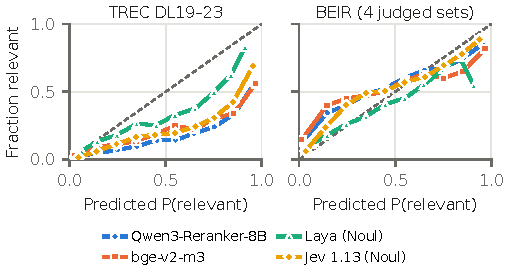
\includegraphics[width=0.8\textwidth]{figures/reliability.pdf}
\caption{Raw reliability on judged candidate pairs for bge, Qwen3-Reranker-8B, and the Noul readouts of Laya and Jev. Pooled within DL19--23 (left) and the four BEIR collections with negatives (right); 10 equal-width bins for readability (the ECE values in Table~3 of the main article use 15 bins), hiding bins with fewer than 15 pairs. Noul needs no strict/lenient policy choice. Decision models are closer to the diagonal on DL and, pooled, on BEIR, though less uniformly across BEIR collections.}
\label{fig:reliability}
\end{figure}

\subsection{Neural first stage}\label{app:first-stage}

To check whether the system ordering depends on BM25, we reranked RankLLM's SPLADE++ EnsembleDistil~\cite{formal2022spladepp} top-100 candidates for DL19 and DL20 (same qrels) with bge-reranker-v2-m3, MiniLM, Qwen3-Reranker-8B, and Jev's three formats. SPLADE++ alone reaches 73.1/72.0 nDCG@10 on DL19/DL20 (BM25: 50.6/48.0), so every reranker gains much less. bge-reranker-v2-m3 scores 76.0/75.6, Qwen8B 75.5/73.1, and MiniLM 74.9/74.4. Jev scores 70.5--72.9 on DL19, 3.1--5.5 points below bge (Score-4: $p=0.03$, unadjusted) and below the SPLADE++ ranking itself, whereas on BM25 candidates it was within 1.1 points of bge. On DL20 it scores 74.6--77.1, and Noul is the best system (77.1, $+1.5$ over bge, $p=0.50$). Jev, however, places more unjudged candidates in its top 10 than the cross-encoders do (Judged@10 86.7--87.9\% on DL19 versus 94.9\% for bge and 94.2--94.7\% for Qwen8B and MiniLM; 90.9--91.9\% versus 97.6\% for bge on DL20), and standard nDCG@10 counts them as non-relevant. On condensed lists, which drop unjudged candidates before scoring~\cite{sakai2007alternatives}, Jev's DL19 gap to bge shrinks to $-0.1$ to $-1.7$ points (none significant), Jev is no longer below the SPLADE++ ranking (76.0--77.5 versus 75.9), and on DL20 it leads bge by $+3.0$ to $+4.0$ (Noul $p=0.04$, unadjusted). Neither scoring bounds the difference under complete judgments: standard scoring counts unjudged candidates as non-relevant and condensed scoring removes them, but an unjudged candidate could carry any grade. Setting every unjudged candidate in the two top-10 lists (1.8 per query on average) to grade 1, 2, or 3 gives a Jev S4 minus bge difference of $-1.8$, $+1.5$, or $+4.0$ on DL19, and the exact range over all completions is $[-8.7,+7.8]$. The DL19 deficit therefore cannot be separated from incomplete judgments, and even its sign is not established. The BM25 pools are also less complete for Jev (Judged@10 90.5--93.5\% versus 96.0--97.2\% for bge); there, condensed scoring moves Jev's DL19 difference to bge from $-1.0$ to $+0.5$ to between $+0.9$ and $+1.8$ points (not significant).

\subsection{Split and provenance audit}

Calibration, pilot, and final question IDs are disjoint, but MuSiQue families overlap substantially. Comparing \texttt{question\_decomposition[-1].id}, 494 final questions share the terminal sub-question with pilot, 349 with calibration, 265 with both, and 578 with either. Comparing any decomposition ID gives 593 pilot overlaps, 430 calibration overlaps, and 671 with either (352 with both). Counts are affected final questions, not unique IDs or matching pairs. The earlier whole-question normalization check found one pilot/final duplicate but missed component reuse. The local component audit checks the source hash and all six cached ranker split-ID sets; its CSV records question-level memberships. The 329-question sensitivity excludes any directly shared component, yet 23 questions in 18 source-graph families remain indirectly connected to design questions. It therefore cannot establish fully family-disjoint generalization. The audit and sensitivity scripts preserve the original splits and model outputs. The reproduction manifest records complete input SHA-256 hashes, all split IDs (including the family-disjoint splits), installed package versions, analysis-source hashes, and the run-manifest hash, and links the component and family-disjoint audits. Historical Hugging Face weight commits were not recorded; architecture strings cannot recover exact weight revisions. Original cached outputs should be preserved for historical numerical verification.


\bibliographystyle{sn-basic}
\bibliography{refs}
\end{document}
